\hypertarget{allvars_8h}{\section{allvars.\-h \-File \-Reference}
\label{allvars_8h}\index{allvars.\-h@{allvars.\-h}}
}


declares global variables.  


{\ttfamily \#include $<$stdio.\-h$>$}\*
{\ttfamily \#include $<$gsl/gsl\-\_\-rng.\-h$>$}\*
{\ttfamily \#include \char`\"{}tags.\-h\char`\"{}}\*
\-Include dependency graph for allvars.\-h\-:
\nopagebreak
\begin{figure}[H]
\begin{center}
\leavevmode
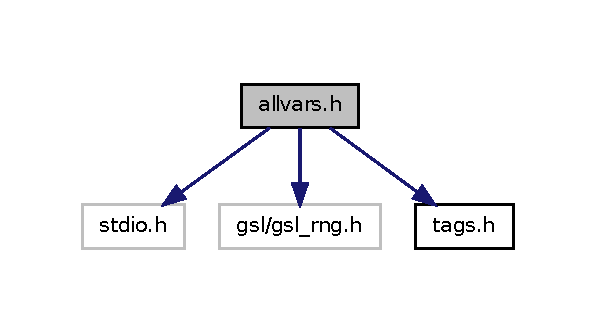
\includegraphics[width=286pt]{allvars_8h__incl}
\end{center}
\end{figure}
\-This graph shows which files directly or indirectly include this file\-:
\nopagebreak
\begin{figure}[H]
\begin{center}
\leavevmode
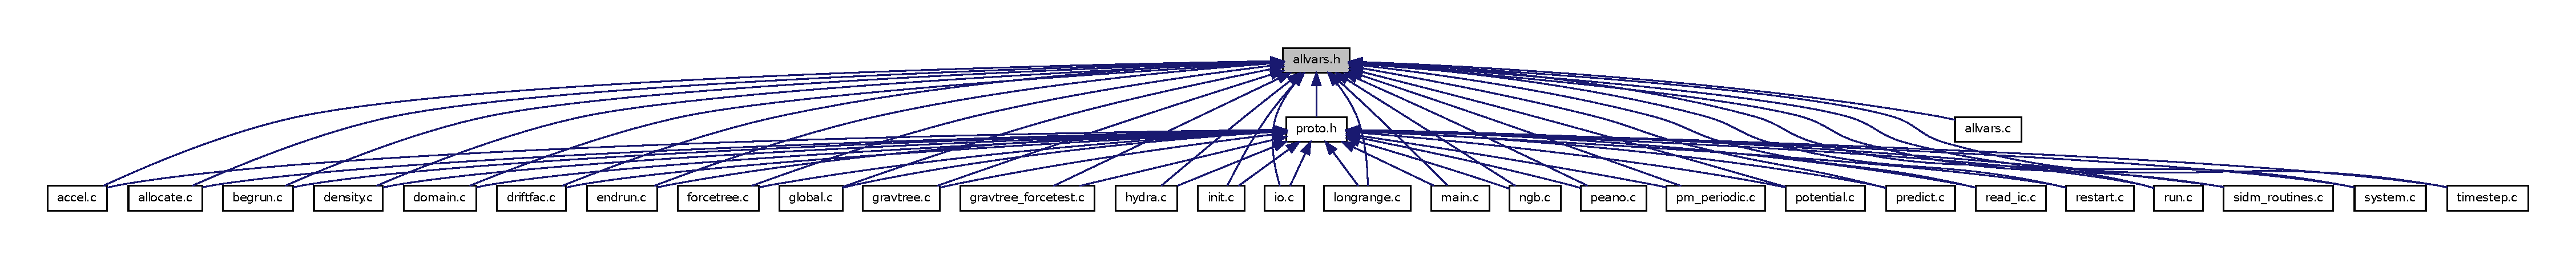
\includegraphics[width=350pt]{allvars_8h__dep__incl}
\end{center}
\end{figure}


\subsection{\-Detailed \-Description}
declares global variables. \-This file declares all global variables. \-Further variables should be added here, and declared as 'extern'. \-The actual existence of these variables is provided by the file '\hyperlink{allvars_8c}{allvars.\-c}'. \-To produce '\hyperlink{allvars_8c}{allvars.\-c}' from '\hyperlink{allvars_8h}{allvars.\-h}', do the following\-:


\begin{DoxyItemize}
\item \-Erase all \#define's, typedef's, and enum's
\item add \#include \char`\"{}allvars.\-h\char`\"{}, delete the \#ifndef \-A\-L\-L\-V\-A\-R\-S\-\_\-\-H conditional
\item delete all keywords 'extern'
\item delete all struct definitions enclosed in \{...\}, e.\-g. \char`\"{}extern struct global\-\_\-data\-\_\-all\-\_\-processes \{....\} All;\char`\"{} becomes \char`\"{}struct global\-\_\-data\-\_\-all\-\_\-processes All;\char`\"{} 
\end{DoxyItemize}

\-Definition in file \hyperlink{allvars_8h_source}{allvars.\-h}.

